\chapter{System Architecture and Load Distribution}

In this project, six nRF52840 devices are employed to implement the testing of a fully automated sowing system. These devices are specifically organized into roles for sensors and actuators to ensure efficient communication, data collection, and actuation. The system is designed to optimize task distribution across devices while maintaining scalability and performance.

The system architecture is composed of the following elements


\begin{figure}[H]
    \centering
    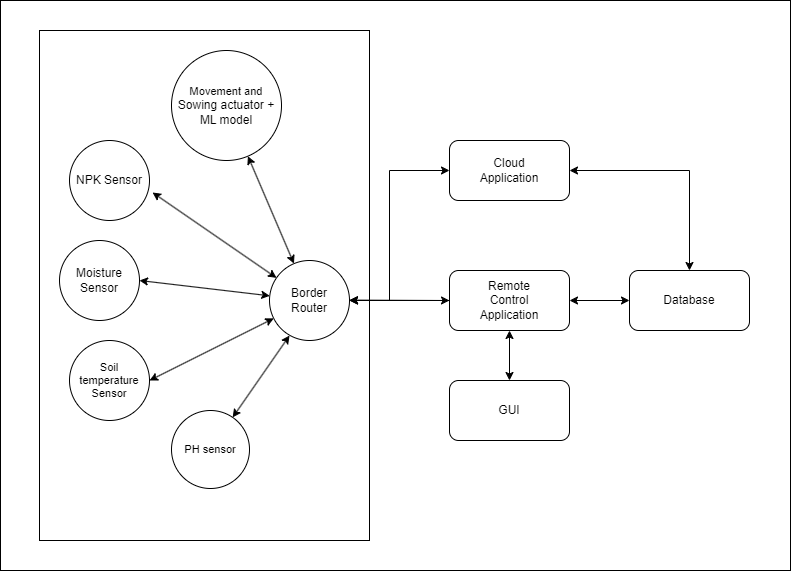
\includegraphics[width=0.5\textwidth]{media/IoT_architecture.png}
    \caption{SeedBot Architecture}
    \label{fig:SeedBot Architecture}
\end{figure}

\begin{itemize} 
    \item \textbf{Border Router:} 
    \begin{itemize} 
        \item Acts as the central communication hub, managing all data exchanges between sensors, actuators, and external networks. It handles routing, ensuring efficient data transmission, and maintains the network's topology.
    \end{itemize} 
    \item \textbf{Sensors:} 
    \begin{itemize} 
        \item \textbf{NPK Sensor:} Measures the soil's nitrogen, phosphorus, and potassium levels. 
        \item \textbf{Moisture Sensor:} Monitors soil moisture levels to ensure optimal growing conditions. 
        \item \textbf{PH Sensor:} Measures the soil pH levels, helping optimize the sowing conditions based on acidity or alkalinity. 
        \item \textbf{Temperature Sensor:} Collects soil temperature data to help in seed germination analysis. 
    \end{itemize} \item \textbf{Actuator:} 
    \begin{itemize} \item \textbf{Movement and Sowing Actuator:} Controls the robot’s movement and seed distribution. Decisions are made based on input from the machine learning model to ensure efficient sowing. 
    \end{itemize} \item \textbf{Applications:} 
    \begin{itemize} \item \textbf{Cloud Application:} Handles the storage and processing of sensor data in a central database. 
        \item \textbf{Remote Control Application:} Provides a graphical user interface that allows users to remotely control the system and monitor real-time data. 
    \end{itemize} 
\end{itemize}

This balanced division of labor ensures that the workload is effectively shared among the devices, allowing the system to operate smoothly and in real-time while minimizing latency and maximizing resource utilization.